\chapter{Implementation}
	The most important details of the implementation of the solution as well as the performed tests are documented in this chapter.

	\section{Code Implementation}
		The work between the developers was distributed by using \gls{Kanban} Boards within the \textit{Projects} function in GitHub, it also gave the project manager the ability to track the current status of the project. GitHub (hosted by ZHAW) was also used as the remote repository for the team. \textit{\gls{Azure Pipelines}} and \textit{\gls{SonarCloud}} were used for \textit{\gls{Continous Integration and Deployment}} and ensuring code quality and security respectively. The most recent build of RaceTrack gets automatically built through the use of \textit{Azure Pipelines}.
		\\~\\

		As described in section \textit{Software Architecture}, RaceTrack implements a layered architecture, which can also be taken from the project structure in the source code itself:
		\begin{figure}[H]
			\centering
			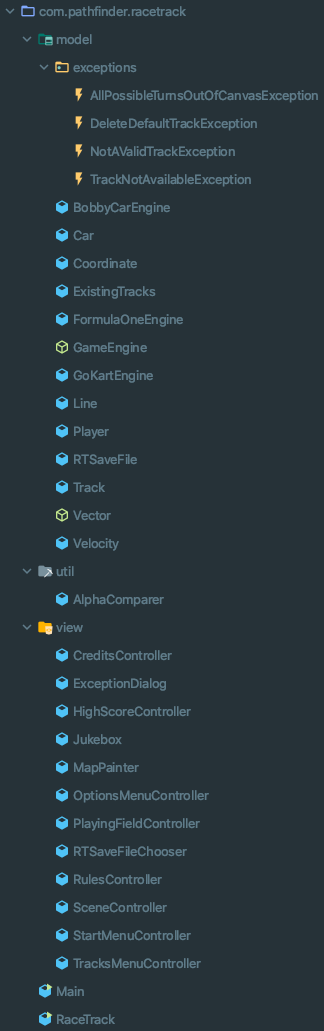
\includegraphics[height=18cm,keepaspectratio,center]{img/Implementation_Code_Package-Structure.png}
			\caption{Java Project Structure of RaceTrack}
		\end{figure}

		\subsection{Packages}

			\subsubsection{com.pathfinder.racetrack.model}
				A \textit{GameEngine} represents the brain of a game session, each game mode (currently three in total) extends the abstract class \textit{GameEngine} with its extensions. There are currently three game modes available.
				\begin{figure}[H]
					\centering
					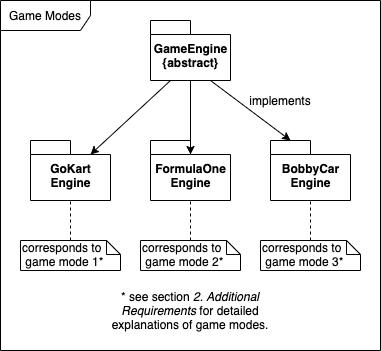
\includegraphics[width=8cm,keepaspectratio,center]{img/Implementation_Code_Game-Modes.png}
					\caption{Implementation Overview of the different Game Modes}
				\end{figure}
				As per layered architecture, the models are being updated in the domain logic, a \textit{GameEngine} in RaceTrack to be exact. But there are still some connections and dependencies between some models themselves: e.g. \textit{Velocity} and \textit{Coordinate} both extend the abstract class \textit{Vector}, which is used by \textit{Car}, which is also owned by a \textit{Player}.
				\begin{figure}[H]
					\centering
					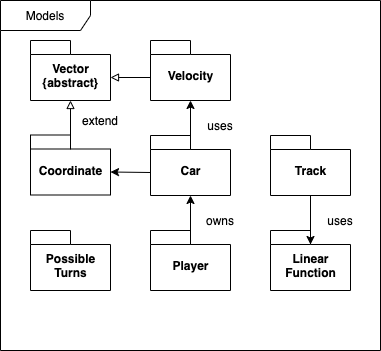
\includegraphics[width=8cm,keepaspectratio,center]{img/Implementation_Code_Models.png}
					\caption{Implementation Overview of the different Game Models}
				\end{figure}

			\newpage

			\subsubsection{com.pathfinder.racetrack.view}
				Player input through the GUI is handled by the \textit{controllers}. Each controller is responsible for a different section of the GUI (e.g. \textit		{StartMenuController} for input in the main menu), except for the \textit{SceneController}, which manages what menu is currently viewed by the player.
				\begin{figure}[H]
					\centering
					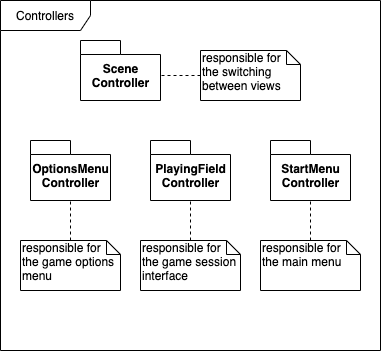
\includegraphics[width=8cm,keepaspectratio,center]{img/Implementation_Code_Controllers.png}
					\caption{Implementation Overview of the different Game Controllers}
				\end{figure}
				The \textit{View} package also holds the classes \textit{Jukebox} and \textit{MapPainter}, which are both only utility classes for the actual user interfaces (\textit{Jukebox} for adding sounds effects and \textit{MapPainter} for drawing the playing field).
				\begin{figure}[H]
					\centering
					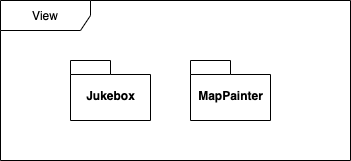
\includegraphics[width=8cm,keepaspectratio,center]{img/Implementation_Code_View.png}
					\caption{Implementation Overview of the View Components}
				\end{figure}
				The actual interfaces are being built by \textbf{JavaFX} through \textit{.fxml} files, which are located in the \textit{resources} directory in the source code.
				\begin{figure}[H]
					\centering
					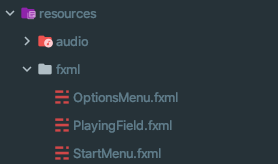
\includegraphics[width=8cm,keepaspectratio,center]{img/Implementation_Code_Resources.png}
					\caption{Implementation Overview of the View Components}
				\end{figure}
